\chapter{Πειραματική Αξιολόγηση}
\label{chap6}

Στο κεφάλαιο αυτό εξηγούμε ότι θα παρουσιαστεί η πειραματική αξιολόγηση και ο έλεγχος σωστής λειτουργίας του αλγορίθμου. 


\section{Παράμετροι αξιολόγησης}

Εδώ περιγράφουμε λεπτομερώς τί παραμέτρους θα μετρήσουμε και εξηγούμε γιατί διαλέξαμε τις παραμέτρους αυτές. 

\section{Σύστημα αξιολόγησης}

Εδώ περιγράφουμε το σύστημα που χρησιμοποιήσαμε για να αξιολογήσουμε τις τεχνικές μας. Συνήθως, η περιγραφή γίνεται με κείμενο και με ένα block diagram περιγραφής των λειτουργιών του συστήματος.
Αν το σύστημα είναι μεγάλο, τότε συζητήστε με τον επιβλέποντα μήπως χρειάζεται να υπάρχει ξεχωριστό κεφάλαιο με τίτλο ` Σχεδίαση συστήματος '. 

\section{Οργάνωση πειραμάτων}

Εδώ περιγράφουμε λεπτομερώς πώς οργανώσαμε τα πειράματα. Π.χ.
α) τί σύνολο δεδομένων χρησιμοποιήσαμε (συνθετικά, έτοιμες συλλογές)
β) τί τιμές είχαν διάφοροι παράμετροι του συστήματός αξιολόγησης, κ.λ.π.

Οι τιμές των παραμέτρων μπορούν να φαίνονται και σε πίνακα, όπως λ.χ. στον Πίνακα \ref{tab:parameters}:

\begin{table}[h]
\centering
\begin{tabular}{|c|>{\centering\arraybackslash}m{8cm}|}
\hline Πλήθος κελιών καννάβου \textit{\tl{c}} $\times$ \textit{\tl{c}} & 50 $\times$ 50, 100 $\times$ 100, 200 $\times$ 200, \textbf{250} $\times$ \textbf{250}, 500 $\times$ 500, 1000 $\times$ 1000  \\
\hline Τυπική απόκλιση $\sigma$ & 25\tl{m}, 50\tl{m}, 75\tl{m}, \textbf{100\tl{m}}, 150\tl{m}, 200\tl{m} \\
\hline Αριθμός εγγύτερων γειτόνων \textit{\tl{k}} & 1, 2, \textbf{3}, 4, 5, 10, 20 \\
\hline Πιθανοτικό κατώφλι $\theta$ & 50$\%$, 60$\%$, 70$\%$, \textbf{75$\%$}, 80$\%$, 90$\%$, 99$\%$ \\
\hline  
\end{tabular}
\caption{Παράμετροι πειραμάτων}
\label{tab:parameters}
\end{table}

Αν χρησιμοποιήσατε συνθετικά δεδομένα, τότε εξηγήστε στην παρακάτω χωριστή υποενότητα τον τρόπο που τα δημιουργήσατε:

\subsection{Παραγωγή συνθετικών δεδομένων}

Τα πειραματικά δεδομένα παρήχθησαν ...


\section{Αποτελέσματα της μελέτης}

Εδώ παρουσιάζουμε τα αποτελέσματα των μετρήσεων με μορφή γραφικών παραστάσεων, όπως ενδεικτικά στο Σχ. \ref{GridGranularity}. Δίνουμε λεπτομερή εξήγηση και σχολιασμό των αποτελεσμάτων, πάντα σε σχέση με το πρόβλημα που οι τεχνικές μας φιλοδοξούν να λύσουν. 
Φροντίστε να ομαδοποιήσετε τα αποτελέσματα (σε χωριστές υποενότητες)ανάλογα με τις παραμέτρους που μετράτε, π.χ. χωριστά το κόστος σε χρόνο από το κόστος σε χώρο ή όσον αφορά την ακρίβεια των απαντήσεων.

\begin{figure}[t!]
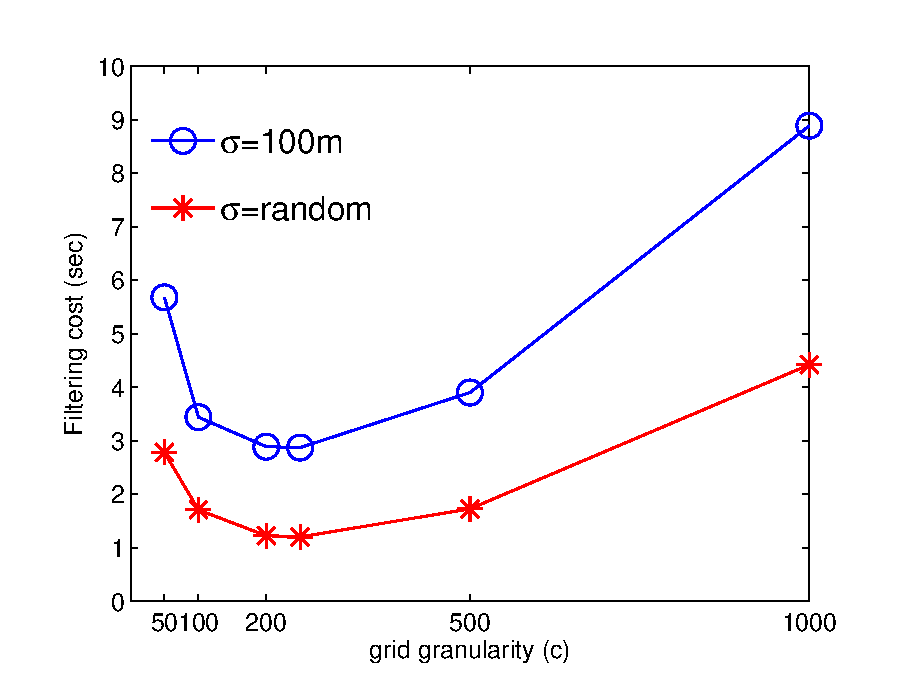
\includegraphics[scale=0.5]{figures/grid_granularity.eps}
\centering
\caption{Κλιμάκωση χρόνου εκτέλεσης για διάφορες υποδιαιρέσεις του καννάβου}	
\label{GridGranularity}
\end{figure} 


\section{Σύνοψη συμπερασμάτων αξιολόγησης}

Εδώ συνοψίζουμε τα συμπεράσματα της αξιολόγησης. Η σύνοψη να γίνεται σύντομα και καθαρά, π.χ. 1. αυτό, 2. το άλλο, κ.ο.κ.

